\chapter{基于生成式对抗网络的多模态图像转换}

多模态图像转换任务可以看作一类特殊的图像转换任务。近些年来,在研究人员的持续努力下,图像转换取得了很大进展,但现有的工作难以对多个输入之间的相关性进行建模,因此多模态图像转换仍非常具有挑战性。在本文中,我们提出了一种新颖的联合注意力生成式对抗网络 (Joint Attention Generative Adversarial Networks,JAGAN) 框架,通过可用的多模态图像生成缺失的模态图像。为了更有效地提取与目标模态一致(相关)的多模态表示,我们使用自表示网络来驱动我们提出的联合注意力机制。JAGAN提取的多模态特征可以与目标模态保持通道级的一致性,极大地提高了图像转换性能。通过与现有方法在多模态图像转换任务上定量和定性比较,证明了我们方法的能够生成更精准的缺失模态图像。

\section{引言}

图像处理、计算机视觉和计算机图形学等越来越多的应用开始依赖于多模态图像,如在精准医学领域,脑部核磁共振可以得到T1加权成像(T1)、Gd造影剂成像(T1Gd)、T2加权成像 (T2 )和液体衰减反转恢复序列成像(T2-FLAIR)四种模态~\cite{drevelegas2011imaging},医生希望尽可能结合完整的多模态医学图像来做出更精确的诊断,但往往受限于实际条件(医疗条件有限、扫描时间不足以及成本/支出/资源等限制),在多模态数据获取过程中可能出现系统误差,甚至部分模态的缺失~\cite{tanenbaum2017synthetic}等情况。这些不可用的模态图像可能会导致医生决策出现偏差。

由于我们在实践中经常会遇到低质量甚至缺失的模态图像,如何利用已有的、完整的模态图像数据对不可用的模态进行填补,已成为计算机视觉和图像处理中的一个重要研究课题。除了可用的图像数据外,医生还可以使用填补的缺失模态数据辅助决策。

对多模态图像数据中缺失的模态进行填补可以看作是一个图像转换问题。图像转换指将图像从一个图像域转换到另一个图像域,类似的任务包括风格转移、分割、去模糊、超分辨率等。不同图像域指的是光照条件、面部表情、传感器等之间的各种成像差异。研究人员为研究有效的图像转换算法投入了大量精力,并在基于生成对抗网络的方法上取得了重大进展,例如Pix2Pix~\cite{pix2pix}、CycleGAN~\cite{cyclegan}和StarGAN~\cite{stargan}等。然而,这些方法仅适用于单一模态输入,在模型输入与网络设计上并未考虑多模态场景下其他可用模态中包含的有效信息。 CollaGAN~\cite{collagan} 是少数为多模态设计的图像转换模型之一,Dongwook Lee等人针对多模态场景,在CycleGAN的基础上提出多重循环一致性损失,从而实现了从任意多模态输入生成目标模态图像的功能。

CollaGAN的缺点在于没有针对跨模态一致性和模态间互补性进行约束,这使得其不能充分利用输入模型的信息。为了有效地提取目标模态(缺失模态)的多模态表示,充分利用模态间一致性和互补性,我们提出基于联合注意力机制机制的生成对抗网络,用于多模态图像转换。我们从一致性和互补性两个方面约束JAGAN的训练:
对于一致性,我们引入自表示网络,结合我们提出的模态内注意力机制,监督模型在训练过程中从输入模态中提取与目标模态一致的特征;
对于互补性,我们设计了模态间注意力:根据模态间互补性以输入模态的信息补充生成目标模态所需要的信息。模态间注意力需要模态特征之间的兼容性,而这由我们的模态内注意力机制通过一致性约束提供。我们将提出的模态内注意力与模态间注意力机制结合,提出用于多模态图像转换的联合注意力生成式对抗网络。

% 我们提出的框架由转换网络和自表示网络组成。

我们提出基于联合注意力机制机制的生成对抗网络贡献如下:

\begin{enumerate}
\item 我们提出模态间注意力,用于模态间互补性用输入模态的信息补充生成目标模态所需要的信息。
\item 我们引入自表示网络来指导训练期间的生成模型,这提供了模态补充模块所需的特征兼容性,并在特征提取阶段过滤掉无关信息。
\item 通过与现有方法在多模态图像转换任务的定量和定性比较,证明了我们方法的能够生成更精确和逼真的结果。
\end{enumerate}


\section{联合注意力生成式对抗网络}
为了尽可能地提取与目标模态一致的多模态表示,并充分利用模态间互补性,从而提高缺失模态图像的生成质量,我们提出了联合注意力机制,并与自监督学习相结合,提出了一种新的多模态图像转换框架JAGAN。我们提出的JAGAN可以灵活地从可用模态中生成任何缺失的模态。

\subsection{概述}

受多模态相关工作~\cite{zhang2020deep}的启发,我们为多模态图像转换任务提出了模态间互补性和跨模态一致性:
\begin{itemize}
    \item 跨模态一致性:只有与目标模态一致(相关)的特征才能被提取出来,无关的信息的应该被过滤掉。
    \item 模态间互补性:对于多模态任务,大多数模态包含其他模态不包含的信息。可以利用这种性质来估算更好的缺失模态。
\end{itemize}

现有的基于生成式对抗网络的图像转换方法取得了很大进展,但这些方法忽略了可用多模态图像之间的一致性与互补性。对于一致性,我们使用自表示网络,结合我们提出的模态内注意力机制,监督模型在训练过程中从输入模态中提取与目标模态一致的特征。对于互补性,由于目前多模态图像转换任务缺乏大规模数据集,这使得网络很难自动学得如何最大程度地利用模态间互补性。为了解决这个问题,我们提出了模态间注意力,用从其他输入模态中提取的特征来补充生成目标特征所需的特征。

如图~\ref{f1}所示,我们的JAGAN由自表示网络和转换网络组成,转换网络由GANs实现。来自模态$\{m_1, m_2, m_3\}$的输入图像$\{x_1, x_2, x_3\}$分别被送入转换网络对应的分支,来生成目标模态$m_4$的图像$x_4$。我们结合模态内注意力和模态间注意力提取生成模态目标所需特征,模态内注意力受自表示网络监督。出于模态间的互补性,模态间注意力在特征融合之前每个输入模态补充来自其他模态信息。考虑到自编码器强大的自表示能力,我们在此采用自编码器网络作为自表示网络来引导模态内注意力的训练,约束生成器在特征提取阶段只提取与目标模态一致(相关)的特征,这进一步为模态间注意力提供必要的模态特征兼容性。

\begin{figure}
    \centering
    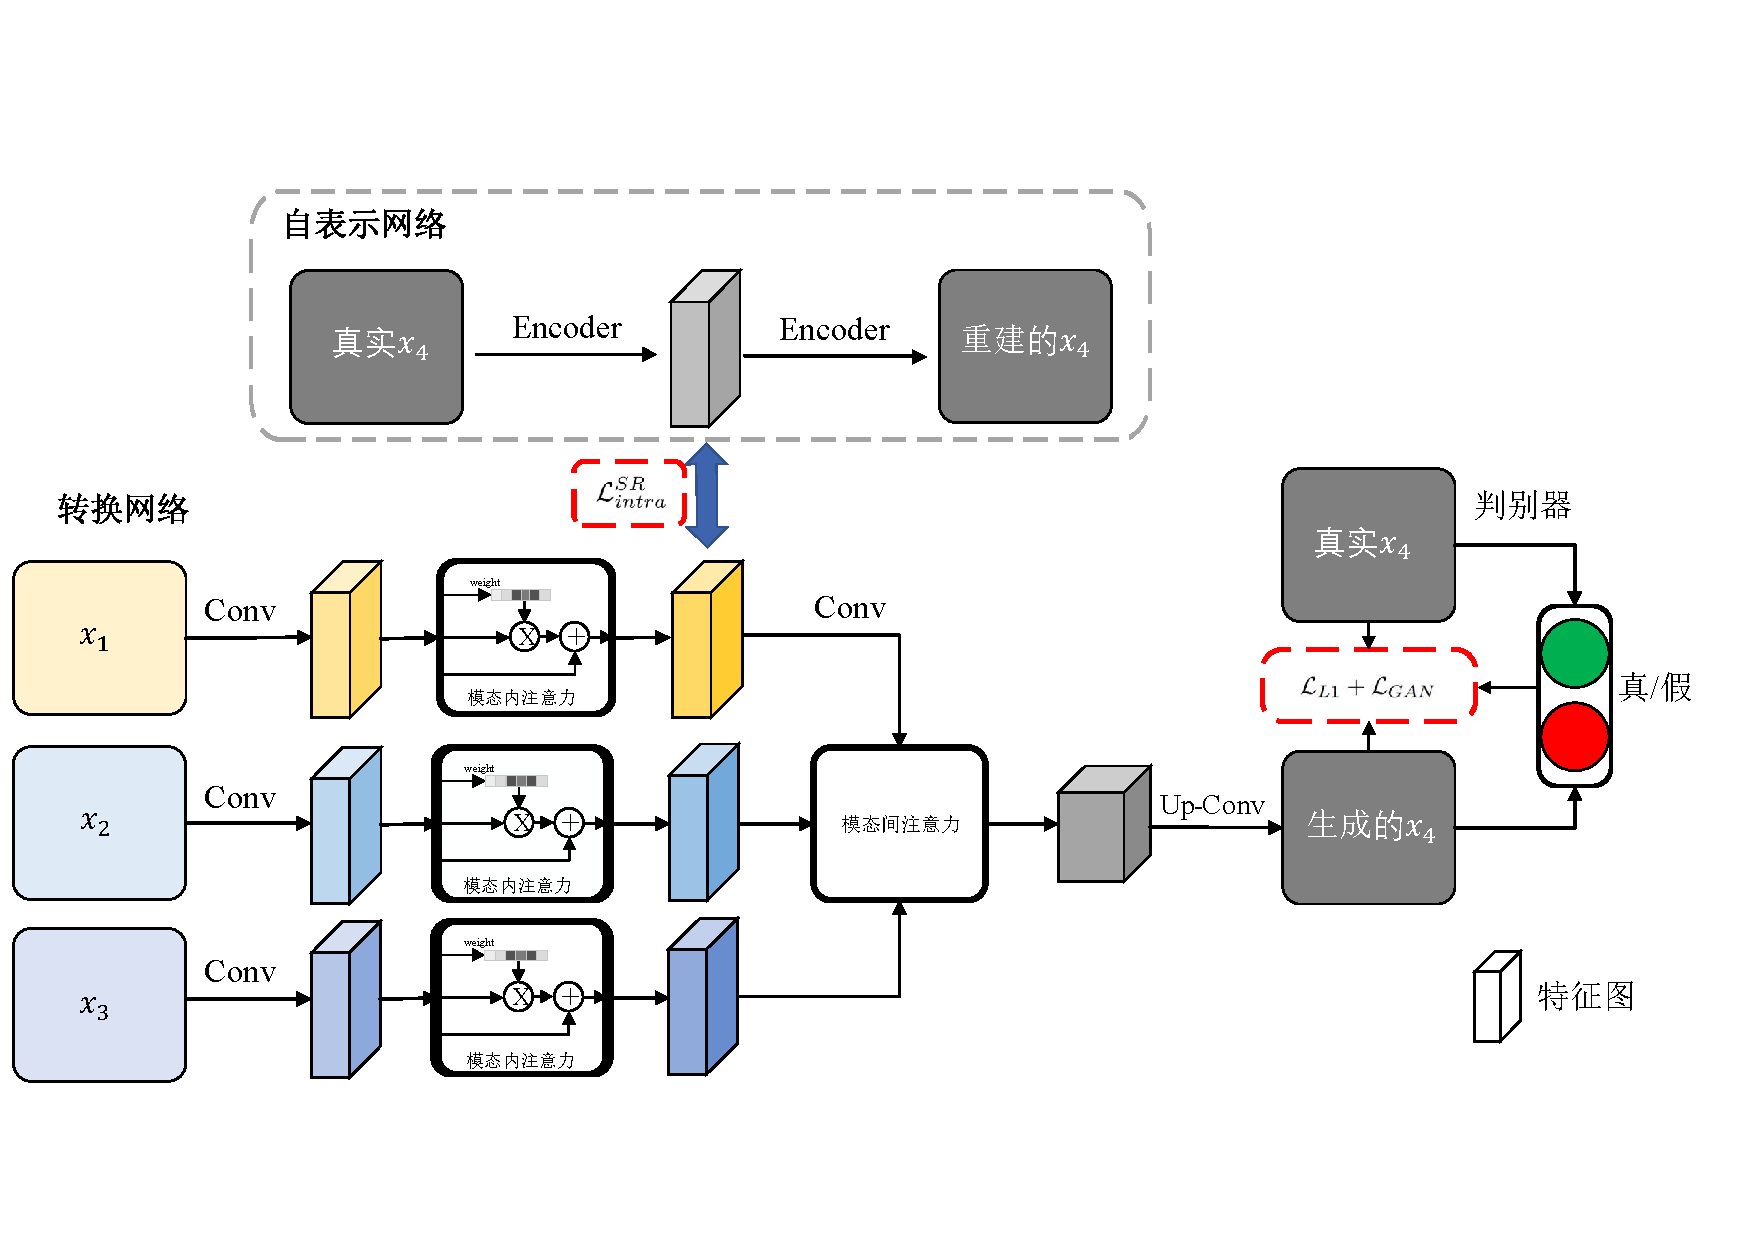
\includegraphics[width=1\columnwidth]{figures/JAGAN/framework.pdf}
    \caption[aaa]{JAGAN框架图}
    \label{f1}
\end{figure}

不失一般性,为了便于表示,我们假设数据集中存在四种模态 $\{m_1, m_2, m_3, m_4\}$。对于转换网络,我们假设模态 $\{m_1, m_2, m_3\}$ 中的输入图像 $\{x_1, x_2, x_3\}$ 被转换为目标模态 $m_4$ 中的目标图像 $x_4$。

\subsection{模态内注意力与自监督学习}

正如我们前面提到的,我们引入了一个自编码器来驱动转换网络$\mathcal{T}$的训练,它由一个带有多分支编码器和单个分支解码器的生成器$\mathcal{G}$和判别器$\mathcal{D}$组成,自表示网络$SR$由自编码器实现。

$SR$ 以通道为粒度驱动 $\mathcal{T}$ 进行训练:
\begin{align}
	\mathcal{L}_{SR} = \sum_{k=1}^n \|f^{SR}_{x_i}- E^{SR}(x_{m_4})\|_2
\end{align}

其中 $E^{SR}(x_{m_4}$表示自表示网络编码器的输出,$f_{x_k}=E_k(x_k)$,$E_k(\cdot)$ 表示生成器$G$第$k$个编码分支$E_k$的输出。

\subsection{模态间注意力}

特征图中的每个通道都可以看作是深度神经网络从输入中提取的某种模式。对于任意通道而言,每个输入模态中包含的信息是不同的。我们仍以医学图像为例,如果第k个通道是关于肿瘤的纹理特征,显然T1Gd包含最丰富和最有价值的信息;如果该通道是关于脑脊液的,那么T2是最重要的模态。一个自然的想法是将T1Gd中的肿瘤相关信息添加到T2模态中,并将T2中的脑脊液相关信息添加到T1Gd模态中。这实际上就是在利用模态间的互补性。

请注意,在向其他模态补充信息之前,对于给定的通道或模式,我们需要知道哪种模态包含最丰富的信息,或者我们需要更多关注哪种模态。受注意力机制~\cite{seq2seq,attentionallyouneed,nonlocal,sagan}的启发,我们提出了一种如图~\ref{f2}所示的模态注意力机制,图中FC表示公式\ref{e1}中定义的两层全连接层,来计算跨模态的通道权重(表示为 $\mathcal{A}$)。

\begin{figure}
	\centering
	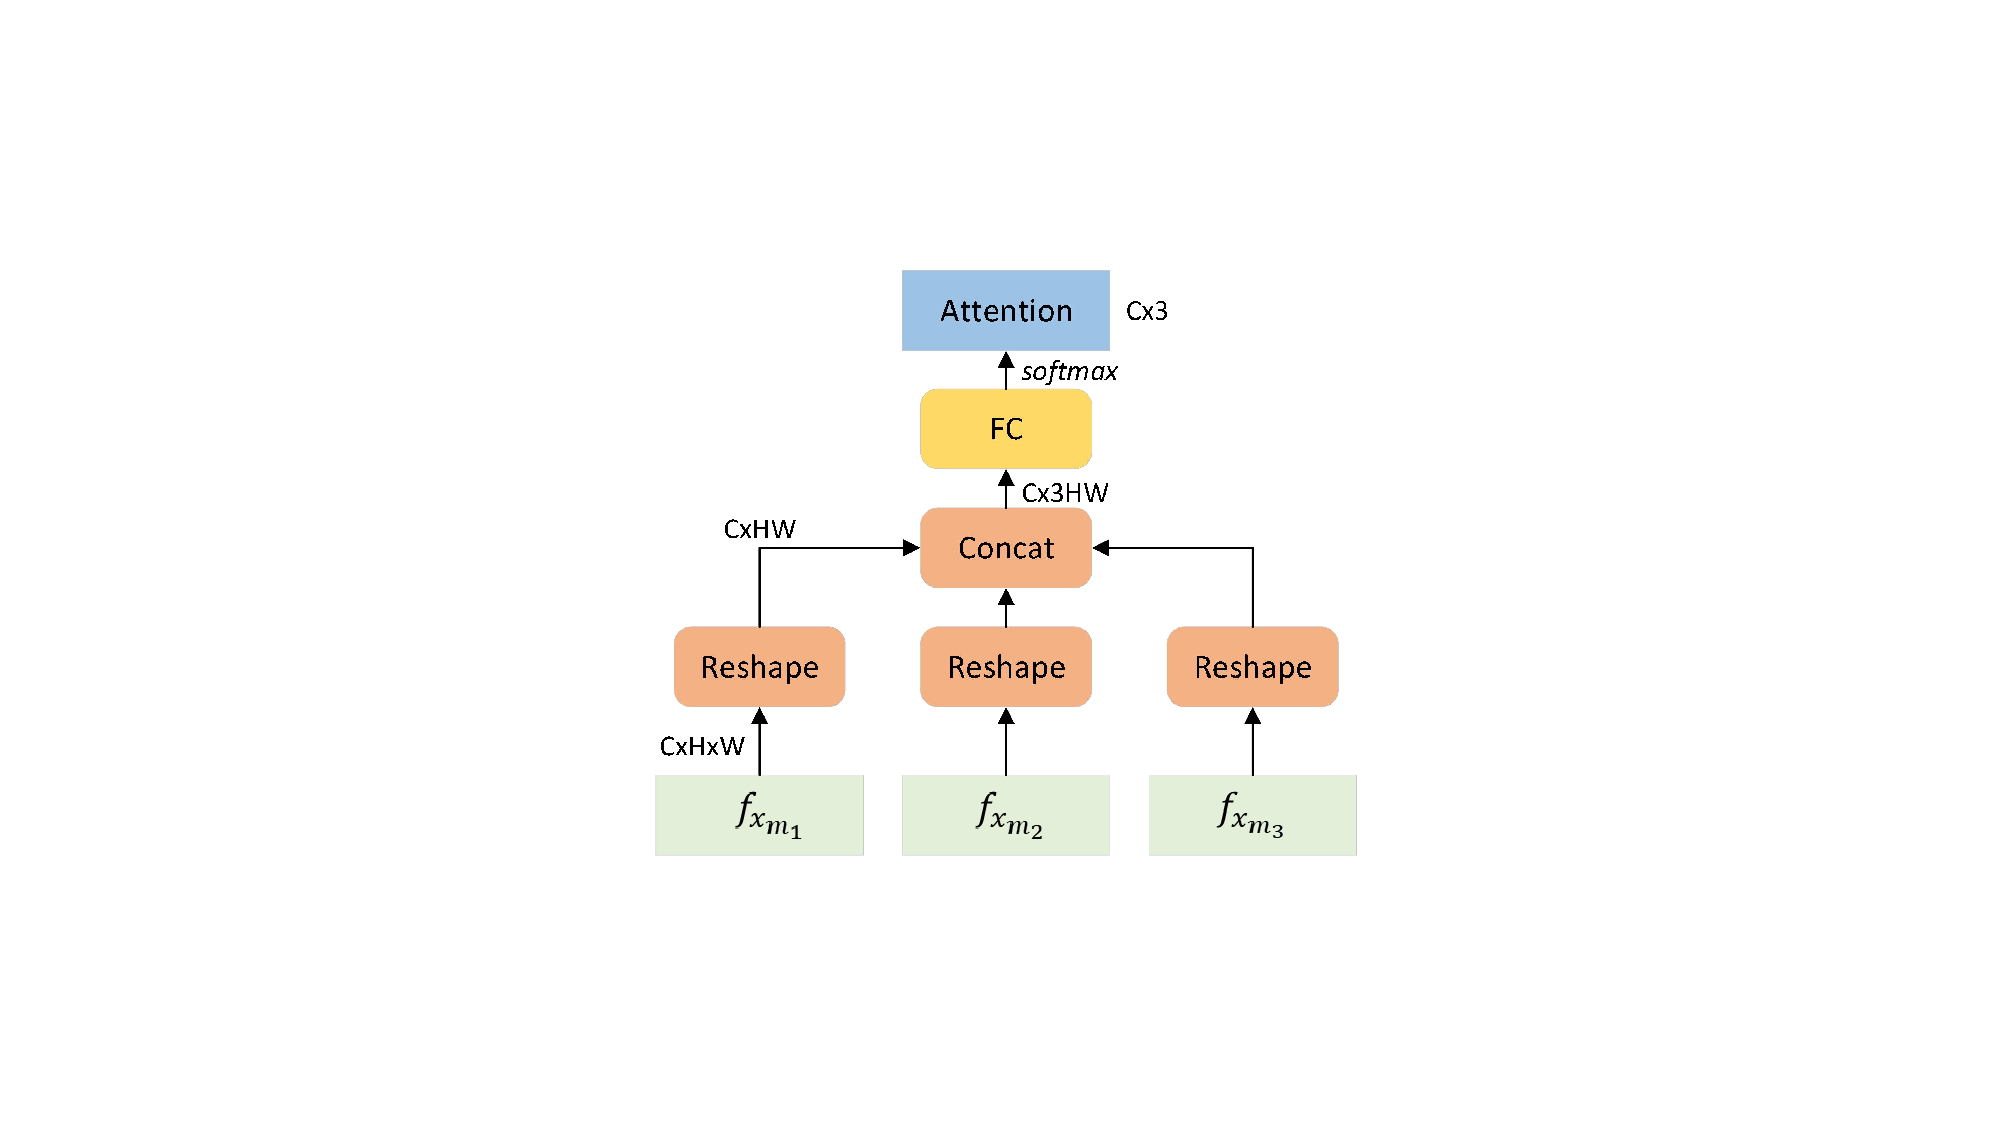
\includegraphics[width=0.8\columnwidth]{figures/JAGAN/20201109InterAttention_function_AV1_0.pdf}
	\caption[]{模态间注意力机制的注意力矩阵计算过程}
	\label{f2}
\end{figure}

\begin{align}
	\mathcal{A} = S_2(\sigma((\delta([f_{x_1}, f_{x_2}, f_{x_3}]W_1))W_2))\
	\label{e1}
\end{align}

其中 $f_{x_k}=E_k(x_k)$,$E_k(\cdot)$ 表示生成器$G$第$k$个编码分支$E_k$的输出,$[\cdot,\cdot]$ 表示张量reshape(将张量从CxHxW展平至CxHW)和串联。 $W_1$和$W_2$是两个全连接层,如图~\ref{f2}。$\delta$和$\sigma$ 分别是ReLU\cite{nair2010rectified}和Sigmoid 函数。 $S_2$是 对$\mathcal{A}$ 每一行进行softmax运算的函数。从结果上来看,元素$\mathcal{A}_{i,j}$第$i$个模态对第$j$个的模态的注意力,换句话说,是用第$j$个的模态向第$i$个模态补充信息时的权重。

如图\ref{fig:Complementary}所示,我们使用$\mathcal{A}$将其他模态的信息补充到每个输入模态中,$A_{i,j}$是$A$第$i$行第$j$的元素. 在上图中,第2种模态以权重$A_{3,2}$向第1种模态的第3个通道补充信息,第3种模态以权重$A_{3,3}$向第1种模态的第3个通道补充信息。通过这种方式,我们可以获得生成$i$-th模态所需的的互补特征$f_{x_i}^{comp}$:
\begin{gather}
	f_{x_i}^{comp} = \gamma * f_{x_i} +
	(1-\gamma) * \sum_{k=1}^n (f_{x_k} * \mathcal{A}_{k})\
\end{gather}
其中$*$表示向量和特征图之间的通道乘法,n输入模态数(在我们前面的假设下这个数字是3)。$\mathcal{A}_{k}$是注意力权重矩阵$\mathcal{A}$的第$k$ 列。在补充信息的同时,通过设置权衡参数$\gamma$来保留当前模态的信息。

\begin{figure}
	\centering
	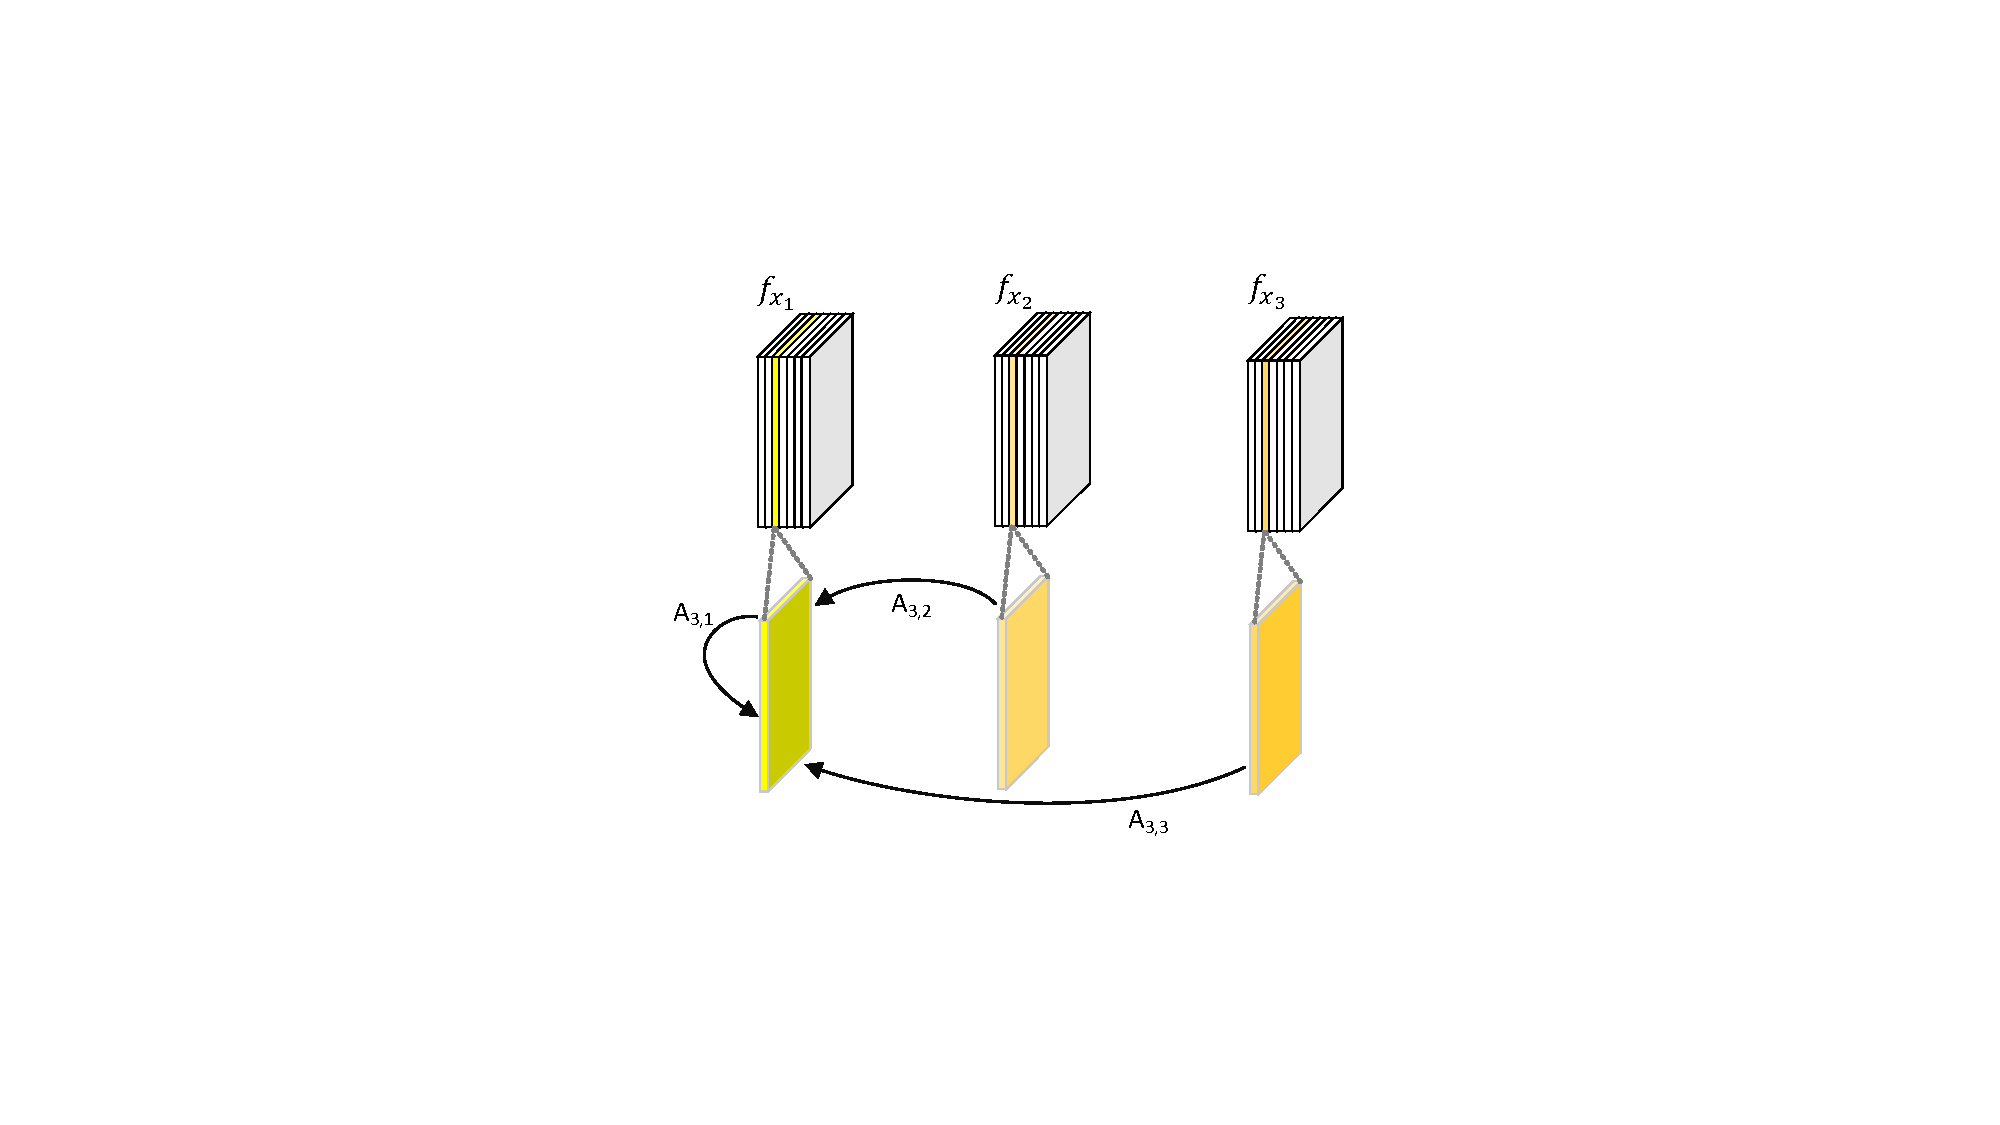
\includegraphics[width=0.8\columnwidth]{figures/JAGAN/20201109InterAttention_function_BV1_0.pdf}
	\caption[aaa]{信息互补的过程} 
	\label{fig:Complementary}
\end{figure}

\subsection{网络实现}

JAGAN由转换网络和子表示网络组成。

\textbf{网络损失} 在训练阶段,我们使用 Adam 来优化模态间注意力-GAN 的生成器 G 的总损失:
\begin{align}
	\mathcal{L}_G = \mathcal{L}_{L1} + \mathcal{L}_{GAN} + \lambda  \cdot \mathcal{L}_{intra}^{SR}
\end{align}
其中 $\mathcal{L}_{L1}$ 和 $\mathcal{L}_{GAN}$ 都是在 pix2pix 中定义的,$\lambda$ 是 $\mathcal{L}_{intra}^{SR}$ 的权重。

\textbf{转换网络} 转换网络由一个生成器和一个鉴别器组成。 我们采用70 × 70的PatchGANs\cite{pix2pix} 作为我们的鉴别器网络和来自 \cite{perceptual} 的架构用于我们的生成器。该网络包含三个用于特征提取和下采样的卷积,几个用于特征变换的残差块,以及三个用于上采样的卷积。为了适应多模态输入,我们重复构造前三个卷积 $\{Conv_1, Conv_2, Conv_3\}$ $n$ 次,形成一个多分支编码器,其中 $n$ 是输入模态的数量,$ Conv_k$ 表示第 $k$ 个卷积,每个分支以$E_i$表示。 我们将模态内注意力模块添加到 $Conv_2$ 和 $Conv_3$之间,并将模态间注意力 注意力添加到 $Conv_3$之后。为了使模型能够接收任何三种模态作为输入,我们在每个输入图像中添加目标模态的one-hot编码的mask\cite{stargan}\cite{collagan}。

\textbf{自表示网络} 自表示网络采用与生成器相同的网络结构,区别在于没有使用多分支编码器,在计算损失时没有使用 $\mathcal{L}_{GAN}$。我们将原始图像输入到自表示网络中,不添加任何mask。 实验表明,仅使用 $\mathcal{L}_{L1}$ 监督,自表示网络可以快速拟合每个数据集,并在$\mathcal{T}$的特征提取阶段提供有效的监督。


\section{实验}

\subsection{实验设置}

\subsubsection{数据集和评测标准}

\textbf{医学图像转换}
对于多模态医学图像转换任务,我们在 BraTS2020~\cite{bakas2018identifying}数据集上评测我们的方法,该数据集由四种核磁共振 (MR) 成像模式组成:T1加权成像(T1)、Gd造影剂成像(T1Gd)、T2加权成像 (T2 )和液体衰减反转恢复序列成像(T2-FLAIR)。 共有494名受试者患有低级别或高级别胶质瘤。 每个MR图像的大小为 $240\times240\times155$,体积元素大小为 $1\times 1\times 1 mm^3$ 由于这些MR图像是通过不同的临床协议和来自多个机构的各种扫描仪获得的,并且肿瘤实体在不同的方式下具有不同的外观,因此转换任务的难度非常大。

我们遵循BraTS2020数据集中的原始训练集测试集划分协议:369个样本作为训练集,剩下的125个样本作为测试集。

\textbf{面部图像转换}
对于多模态面部图像转换任务,我们在 Radboud Faces Database (RaFD)~\cite{langner2010presentation} 上评测我们的方法,该数据集包含八种面部表情:快乐、愤怒、悲伤、轻蔑、厌恶、中立、恐惧、惊讶;和三个注视方向:向左看、向前看、向右看。 共有67名受试者,其中男性38名,女性19名,儿童10名。

由于 RaFD 数据集的样本数量有限,我们在实验中采用了 10 折交叉验证。即90\%的数据(约 60 名受试者)构成了训练集,测试集包含剩余的 10\%(6 或 7 名受试者)数据。

\subsubsection{实现细节}
所有实验均在 PyTorch 框架下使用 NVIDIA TITAN RTX GPU 完成。我们使用动量参数 $\beta_1 = 0.5$ 和 $\beta_2 = 0.999$ 的 Adam 优化器~\cite{kingma2014adam} 优化网络参数。所有实验的批大小均设置为 1。实验过程中使用的所有图像都是空间对齐的。为了使训练更加稳定,我们先单独训练自表示网络,然后在训练转换网络时加载预先训练好的自表示网络。同时训练自表示网络和转换网络可以达到类似的准确率,但需要更多的迭代次数才能完成。

由于BraTS2020数据集中的 3D MR 图像是根据横向平面扫描的,显然它们仅在水平方向上是连续的。在这里,我们遵循扫描方向,从每个样本中提取多个切片。所有图像都缩放到 $256\times256$,并在将它们放入模型之前将像素值归一化到区间 $[-1, 1]$。超参数 $\gamma$、$\lambda$设置为 $0.5$、$0.1$、$0.1$、$3$ 和 $2$。输入和输出通道数在医学图像转换任务中为 1,在面部表情转换任务中为 3。

\subsubsection{基准方法与评测标准}

我们将我们的方法与三种最先进的基于 GAN 的图像转换方法进行比较:Pix2Pix~\cite{pix2pix}、StarGAN~\cite{stargan} 和 CollaGAN~\cite{collagan}。为了和我们的JAGAN公平比较,所有基准方法的所有结果都是在相同的数据集划分协议下训练和测试的。所有结果均来自作者提供的源代码。我们下面将从定性和定量两个角度,对我们的方法和所有基准方法进行比较。

如何评测转换图像是一个公认的难题~\cite{salimans2016improved},这是因为图像中的每个像素不是独立的,我们应该在图像维度上评测它们。因此,对于定量评测,我们采用结构相似性指标度量(SSIM)~\cite{ssim} 来评测图像级的一致性,使用特征相似性指标度量(FSIM)~\cite{fsim} 来评测特征级一致性。SSIM 和 FSIM 分数由转换后的生成图像(伪图像)及其相应的真实图像计算得出。与多模态医学图像转换任务不同,对于面部表情合成来说,即使是相同的表情也会有很大差异,这使得很难利用 SSIM 和 FSIM 对面部图像进行定量评测。由于面部图像属于自然图像,因此,通过在ImageNet上预训练的分类模型计算得到的 Fréchet Inception Distance (FID)~\cite{fid} 更适合面部图像转换任务。对于定性评测,我们将在实验部分对比我们方法和所有基准方法的多模态图像转换结果。

\subsection{对比实验}

最近提出了各种基于 GAN 的图像转换方法。 在这些方法中,Pix2Pix~\cite{pix2pix} 是一种基于 cGAN 的方法,它是我们模型的基本架构,StarGAN~\cite{stargan} 和 CollaGAN~\cite{collagan} 提出了目标模态掩码向量和循环- 一致损失~\cite{cyclegan} 到多模态图像转换任务。因此,我们在下面的实验中将我们的方法与 Pix2Pix、StarGAN 和 CollaGAN 进行比较。

\subsubsection{MR图像转换对比}
为了评测我们所提出的方法在多模态医学图像转换上的性能,我们用Brats2020训练集中的所有数据来训练自表示网络,并从Brats2020训练集中采样三种模态的所有可能组合,作为转换网络的输入,我们可以通过这三种输入模态生成任何缺失的模态。 Pix2Pix和StarGAN只适合单个输入,考虑到 因为 T2-FLAIR 提供的肿瘤实质和水肿区域明显大于其他三种模态,我们选择 T2-FLAIR 作为输入生成 T1、T1Gd、T2模态,T2-FLAIR模态图像则是从T1Gd模态转换而来。 CollaGAN 遵循与我们相同的实验设置。

图~\ref{fig:comparsion_medical}展示了我们的方法、Pix2Pix、StarGAN 和 CollaGAN 在 BraTS2020 数据库上的比较结果。图中黄色的数字是 SSIM 和 FSIM 分数(用斜线分割), 我们用黄色箭头指出了结果的重点区域。StarGAN和CollaGAN的结果在转换T1Gd、T2和T2-FLAIR时整体观感较差,具体体现在软组织细节不清晰,对比度不准确。虽然 CollaGAN 生成了较好的肿瘤纹理,但结果嘈杂,严重降低了整体观感。 Pix2Pix 在生成 T2 和 T2-FLAIR 方面比 StarGAN 和 CollaGAN 产生更好的纹理细节,但 Pix2Pix 的结果对比不明显。与这些方法相比,我们的 JAGAN 显示出清晰的软组织纹理和明显的肿瘤病变区域。

对于定量评测,我们在每个转换样本的右下角显示了平均 SSIM 和 FSIM 分数。这些报告的评测分数由转换后的图像和相应的真实图像计算得出。现有方法忽略了多模态图像中的互补信息,从而降低了定量分数。我们的 JAGAN 在完整的医学图像转换任务集上取得了最高的 SSIM 和 FSIM 分数。

请注意,由于输入限制,本实验中对 Pix2Pix 和 StarGAN 进行了多次训练。 CollaGAN 占用的计算资源比我们的多得多,但获得的结果却很模糊。作为比较,我们的 JAGAN 可以通过统一模型中的剩余数据生成任何目标医疗模态。该实验中的定量和定性比较通过显示更精确和更现实的结果证明了我们方法的优越性。

\begin{figure}
	\begin{center}
		\includegraphics[width=1\columnwidth]{figures/JAGAN/comparsion_medical.pdf}
	\end{center}
	% \caption{Comparison results of our approach, Pix2Pix, StarGAN and CollaGAN on BraTS2020 database. The yellow numbers are the SSIM and FSIM scores. The arrows point out the remarkable parts of the results. For Pix2Pix and StarGAN, the pseudo T1/T1Gd/T2 figures/JAGAN are translated from a T2-FLAIR image, and the T2-FLAIR image is translated from T1Gd. Our JAGAN generates any target modality by the remaining three modalities.}
	\caption{医学多模态图像转换对比图}
	\label{fig:comparsion_medical}
\end{figure}

\subsubsection{面部表情转换对比}
与上一节所提出的多模态医学图像转换方法评测方法类似,我们取 RaFD 数据集训练集中的所有数据~\cite{langner2010presentation} 来训练自表示网络,并从 RaFD 数据集的训练集中选择七种模态的所有可能组合作为输入转换网络。
然后,我们可以将任何七个面部表情图像转换为目标面部表情。 Pix2Pix 和 StarGAN 的输入设置为面部表情“自然”(neutral),因为自然表情和其他表情的差异最小。 CollaGAN 适用于多个输入,因此,它与我们的共享相同的实验设置。

图~\ref{fig:comparsion_facial}展示了我们的方法、Pix2Pix、StarGAN 和 CollaGAN 在 RaFD 数据集上的比较结果。我们使用红色数字表示FID 分数, 用箭头指出结果的重点区域。 我们的 JAGAN 可以通过其余七种模态生成任何目标模态。由于不同面部表情之间的肌肉运动,图像无法严格对齐,然而Pix2Pix 需要配对数据,因此 Pix2Pix 在这些未对齐的面部表情图像上的转换面部图像包含很大的变形,导致整体外观较差。 StarGAN 和 CollaGAN 适用于未配对数据,因此转换的面部表情较为准确,但纹理细节仍是模糊的。
与上述方法形成对比,我们的方法既能生成准确的表情,又有逼真的细节。

对于定量评测,FID 分数显示在每个样本的左上角。分数越低意味着效果越好。 StarGAN 和 CollaGAN 的转换结果是模糊的,这导致了其FID 分数较高。虽然 Pix2Pix 的结果包含更大的变形,但细节比 StarGAN 和 CollaGAN 更真实。与这些最先进的方法相比,我们的方法以最低的 FID 分数实现了最佳的定量评测。

类似于多模态医学图像转换任务,我们的方法可以通过统一模型中的其他七个面部表情生成任何面部表情。这种多模态面部表情转换实验也证明了所提出的 JAGAN 的有效性。

\begin{figure}
	\begin{center}
		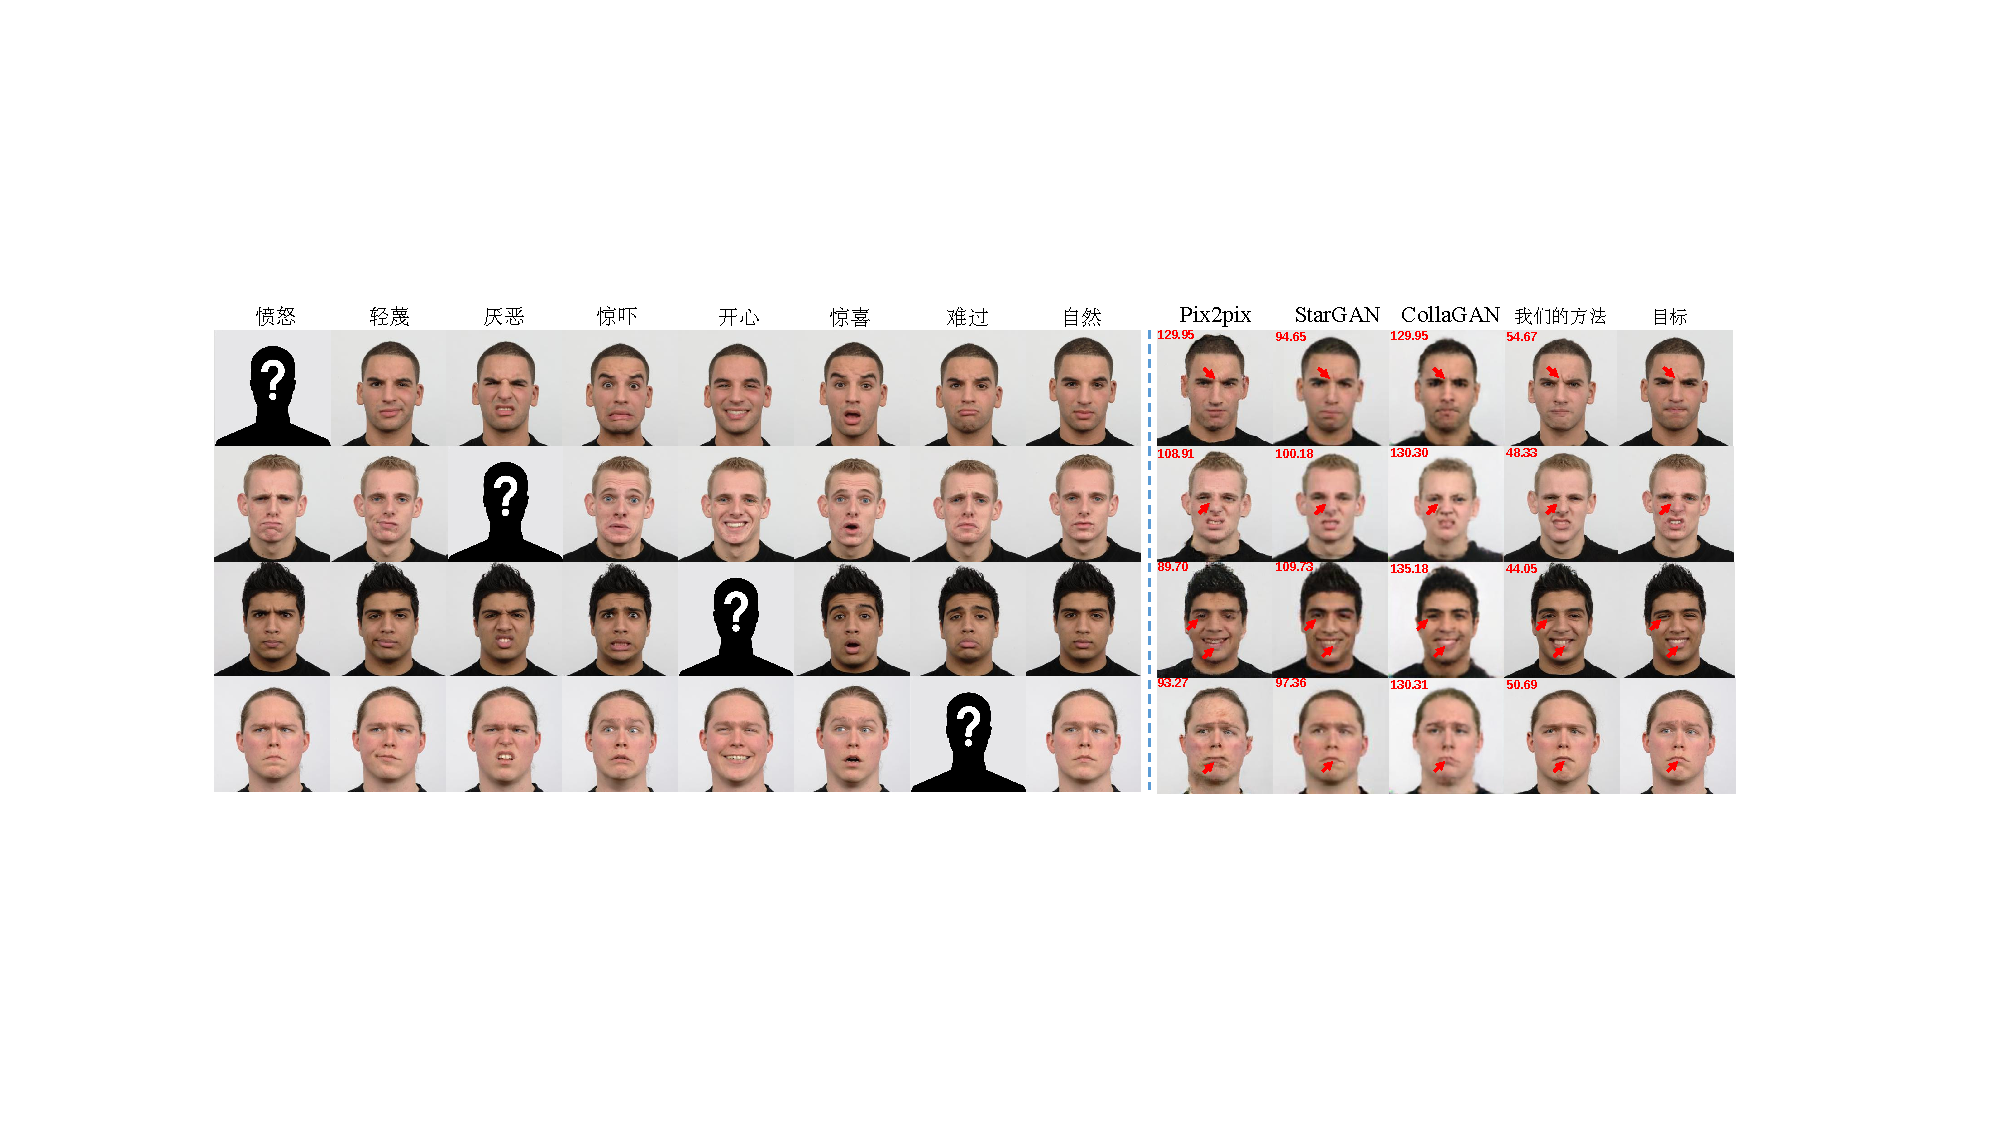
\includegraphics[width=1\columnwidth]{figures/JAGAN/comparsion_facial.pdf}
	\end{center}
	% \caption{Comparison results of our approach, Pix2Pix, StarGAN and CollaGAN on RaFD database. The red numbers are the FID scores. The arrows point out the remarkable parts of the results. For Pix2Pix and StarGAN, the pseudo images are translated from the neutral expression. Our JAGAN can generate any target modality by the remaining seven modalities.}
	\caption{人脸多模态图像转换对比图}
	\label{fig:comparsion_facial}
\end{figure}

\subsection{消融实验}

我们对模态内注意力和模态间注意力进行了消融实验,以量化两个关键模块对整体性能的贡献。以下实验结果表明模态内注意力和模态间注意力都对改进我们的模型有效,我们由模态内注意力和模态间注意力组成的联合注意力为多模态图像转换任务产生了高质量的结果。

我们采用不同的实验设置来验证每个模块的有效性:没有模态内注意力和模态间注意力的 JAGAN、没有模态内注意力的 JAGAN 和没有模态间注意力的 JAGAN。这些方法的一些结果如图~\ref{fig:ablation}所示。
图~\ref{fig:ablation}中:(a)为没有模态内注意力和模态间注意力的JAGAN实验结果,(b)为没有模态内注意力的JAGAN实验结果, (c)为没有模态间注意力的JAGAN实验结果,(d)为JAGAN的实验结果,(e)为真实图像。
图~\ref{fig:ablation}(a)中没有 模态内注意力 和模态间注意力的转换网络生成后的医学图像对比度不准确,肿瘤区域估计也不准确,合成面部表情“轻蔑”更接近“自然”。通过添加模态间注意力,该模型可以更好地估计医学图像的肿瘤区域,以及更准确的面部表情的嘴巴和皱纹,如图~\ref{fig:ablation}(b) 所示。这表明模态间注意力可以有效地融合模态间互补信息。然而,细节并非模糊不清。图~\ref{fig:ablation}(c)是使用模态内注意力模块的基准方法模型的结果,估计的医学图像对比度更准确,面部图像的眼睛等细节纹理更逼真。这验证了模态内注意力可以提供更多的兼容性信息。通过结合 模态内注意力 和模态间注意力,如图~\ref{fig:ablation}(d) 所示,完整的 JAGAN 模型成功地为估计的医学图像生成了最准确的对比度和肿瘤区域,以及最逼真的面部纹理表达转换。

\begin{figure}
	\begin{center}
		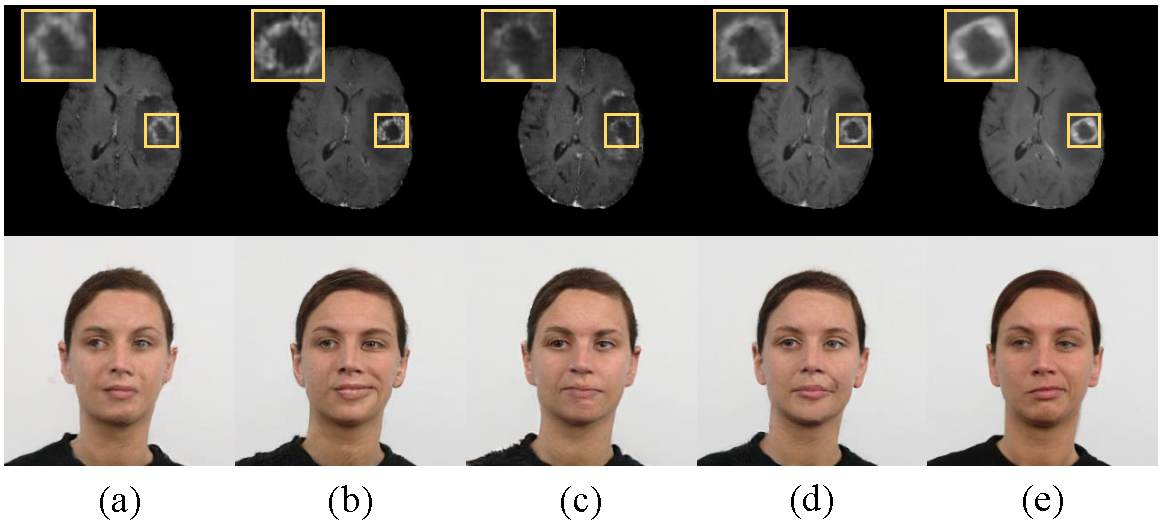
\includegraphics[width=0.8\columnwidth]{figures/JAGAN/ablation.pdf}
	\end{center}
	\caption{消融实验对比图}
	\label{fig:ablation}
\end{figure}

我们接下来探讨采用模态内注意力来保持转换网络中间特征图的目标特定一致性有效性。 如图~\ref{fig:ablation1}所示,在没有模态内注意力的情况下,由相应编码器分支从不同输入提取的特征图差异很大。 在模态内注意力的约束下,从同一个卷积核中提取的特征图满足具有相似外观的跨模态一致性。

\begin{figure}
	\begin{center}
		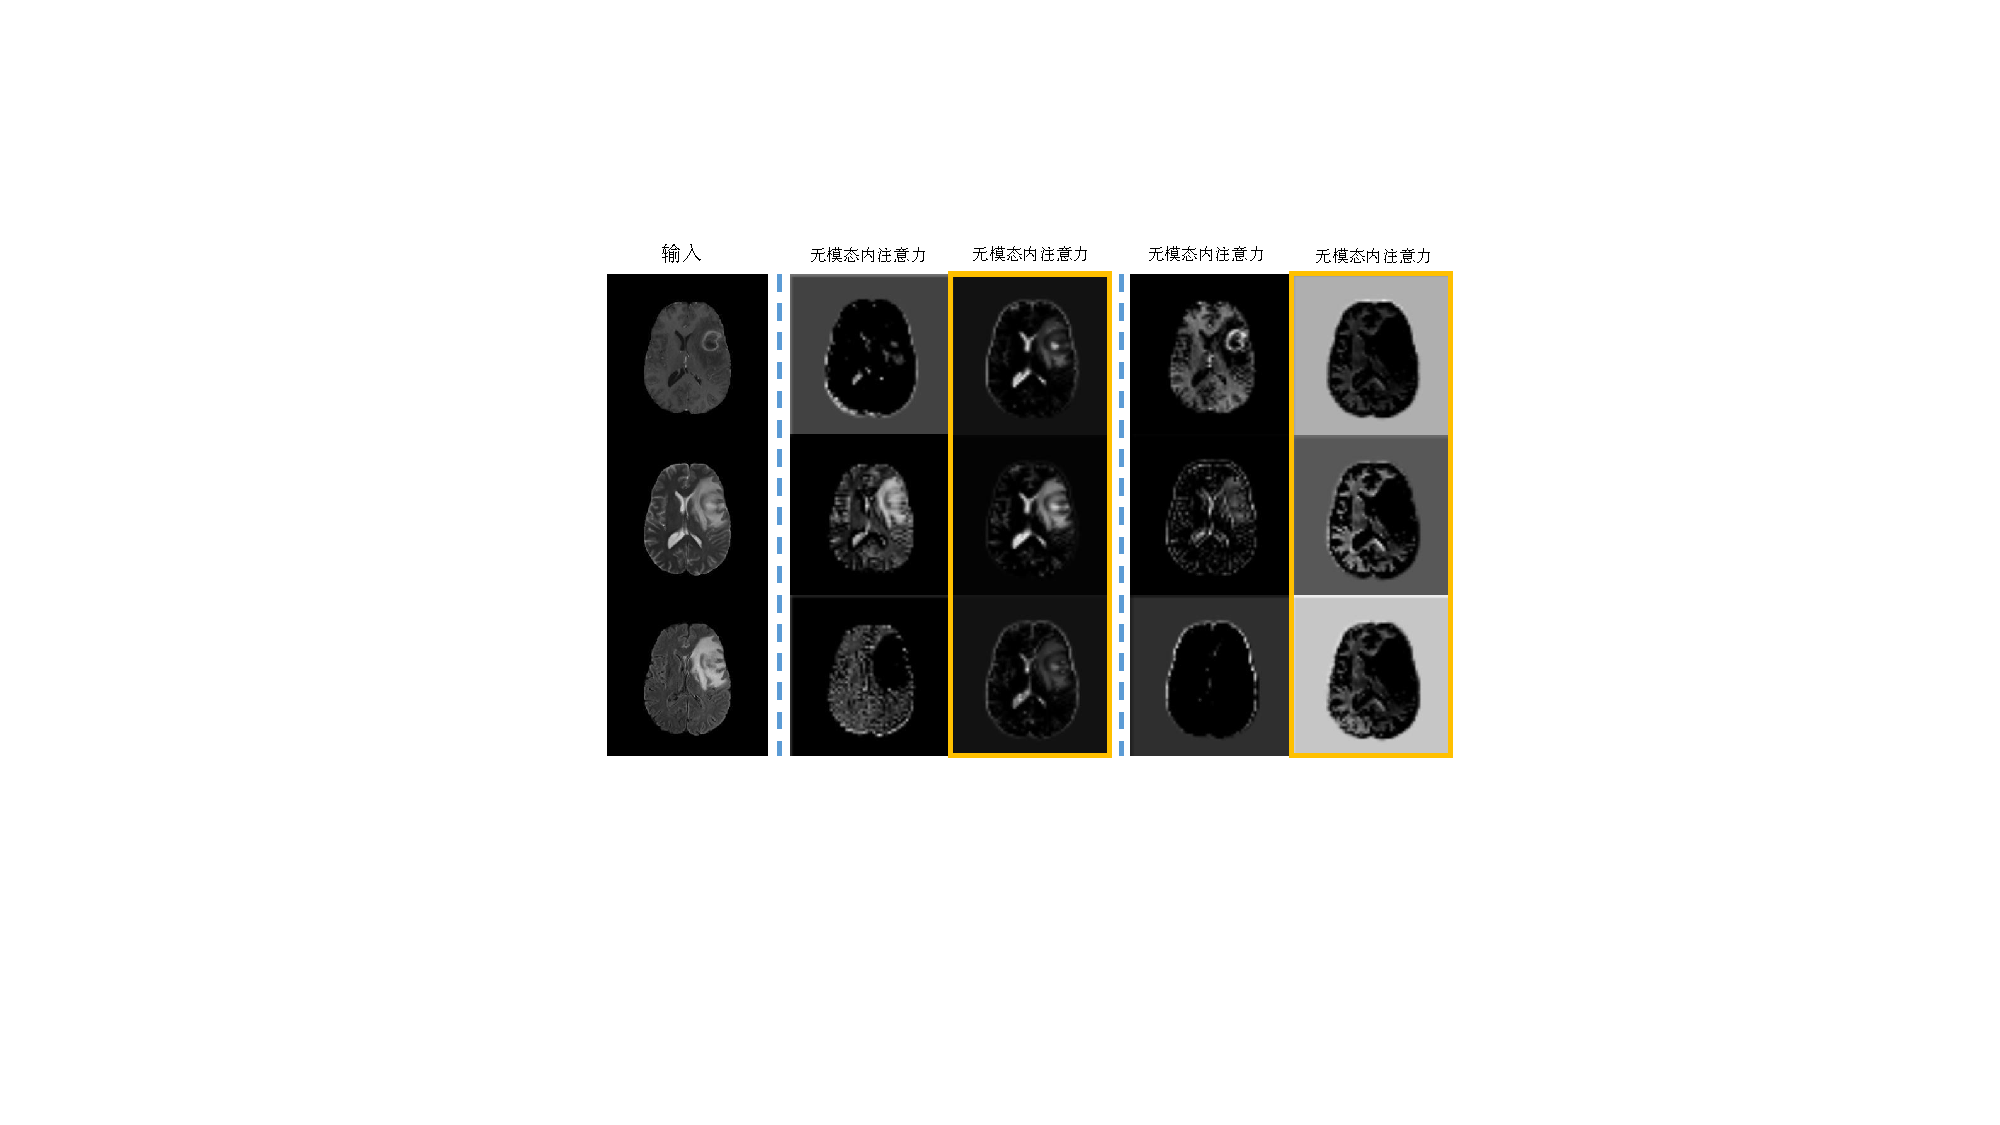
\includegraphics[width=0.8\columnwidth]{figures/JAGAN/ablation1.pdf}
	\end{center}
	\caption{特征图可视化}
	\label{fig:ablation1}
\end{figure}

% 为了定量评测SR网络对转换网络的约束效果,利用t-SNE~\cite{maaten2008visualizing}将提取的特征图嵌入到二维空间中,如图~\ref{fig:regression}。每种颜色代表特征图源自的编码器分支。左子图显示了从没有 SR 网络约束的某个卷积核中提取的特征图的 t-SNE 分布,右子图显示了从同一卷积中提取的特征图的 t-SNE 分布具有 SR 网络约束的内核。我们从每个编码器中选择六个卷积核。对于多模态医疗人物/JAGAN,总共有四组输入和四个编码器。因此,每个子图中有 96 个点。如图~\ref{fig:ablation1}所示,使用SR网络训练的特征图分布比没有SR网络的特征图分布更接近。特征外观和 t-SNE 分布证明了所提出的跨模态一致性的有效性。

% \begin{figure}
%     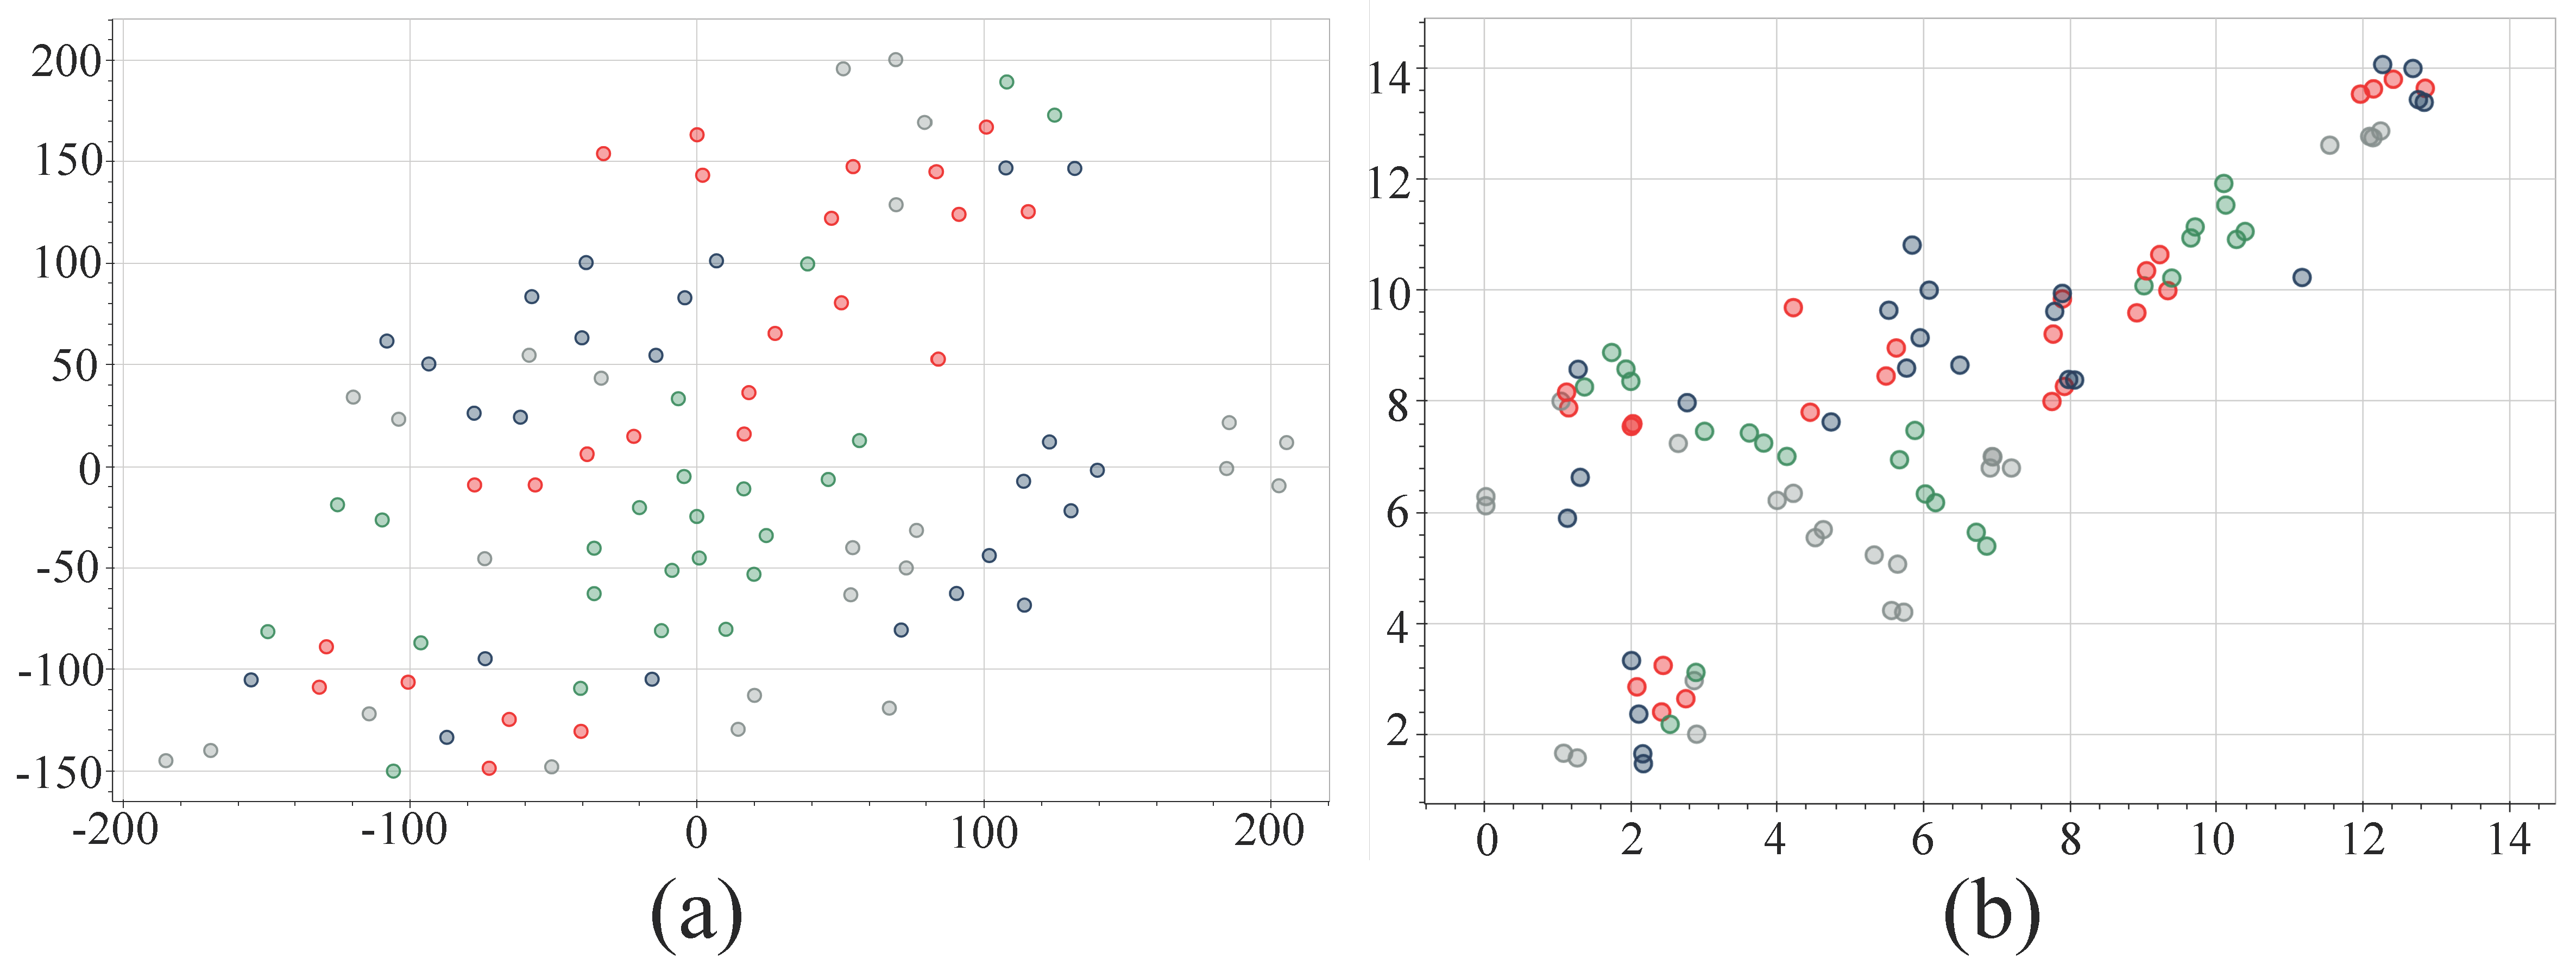
\includegraphics[width=1\columnwidth]{figures/JAGAN/regression.png}
% 	\caption{特征图的二维可视化。每个圆点表示一个特征图,不同的颜色表示其来源自不同的编码器分支。(a)是没有模态内注意力的结果, (b) 则是有模态内注意力的结果。}
% 	\label{fig:regression}
% \end{figure}


\section{本章总结}

在本文中,我们提出了一种用于多模态图像转换的联合注意力 GAN。 我们的方法使用模态内注意力机制为多模态转换网络提供跨模态一致性指导,并为模态间注意力提供兼容性;使用模态间注意力最大化利用模态间互补信息。 我们将模态内兼容性、模态间互补性和跨模态一致性合并到一个统一的生成框架中。设计的多分支编码器和模态掩码向量使我们的 JAGAN 能够在单个统一模型中生成任何缺失的模态,进一步保证其通用性。

虽然我们提出的 JAGAN 与其他最先进的技术相比实现了卓越的性能,但存在一些局限性。例如,在训练阶段,所提出的框架需要更多的计算资源和计算时间。 未来,我们将探索更高效的网络架构。
